\usetikzlibrary{arrows.meta}

\definecolor{bgLight}{HTML}{F8FAFC}
\definecolor{lvlRootBg}{HTML}{4f6fb9}
\definecolor{lvlRootText}{HTML}{F8FAFC}
\definecolor{lvlRootBorder}{HTML}{0284C7}
\definecolor{lvlSectorFill}{HTML}{E0F2FE}
\definecolor{lvlSectorBorder}{HTML}{0284C7}
\definecolor{lvlSectorText}{HTML}{0369A1}
\definecolor{lvlRoleFill}{HTML}{F1F5F9}
\definecolor{lvlRoleBorder}{HTML}{475569}
\definecolor{lvlRoleText}{HTML}{1E293B}
\definecolor{lvlToolFill}{HTML}{CCFBF1}
\definecolor{lvlToolBorder}{HTML}{0D9488}
\definecolor{lvlToolText}{HTML}{0F766E}

\pgfdeclarelayer{bg}
\pgfsetlayers{bg,main}

\newcommand{\nd}[4]{%
  \node[
    draw=#4Border,
    fill=#4Fill,
    text=#4Text,
    line width=1.1pt,
    rounded corners=6pt,
    inner sep=6pt,
    align=center,
    font=\sffamily\bfseries\footnotesize
  ] (#1) at (#2) {#3};%
}

\newcommand{\conn}[5]{%
  \draw[#1Border, line width=#5pt, line cap=round, opacity=0.65] (#2) -- (#3);%
}

\pieDePagina{Metas del ODS \#9. }

% Begin text
\begin{multicols*}{2}
\inicializarSeccion{Objetivo de Desarrollo Sostenible}

\begin{center}
  \includesvg[width=0.8\linewidth]{fase1/SDG9.svg}
  \captionof{figure}{ODS \#9: Industria, innovación e infraestructura.}
  \label{fig:introduccion}
\end{center}

La ODS Seleccionada pretende, construir infraestructuras resilientes, promover la industrialización sostenible y fomentar la innovación.

\vspace{0.5 em}

La industria manufacturera mundial, considerada uno de los motores del crecimiento económico global, ha venido experimentando un declive constante debido a los aranceles y las tensiones comerciales, incluso antes del inicio de la pandemia de la COVID-19. El declive de la industria manufacturera ha tenido graves repercusiones en la economía mundial.

\vspace{0.5 em}

Esto se debe principalmente a la elevada inflación, los cambios en el precio de la energía, las continuas interrupciones en el suministro de materias primas y productos intermedios, y la desaceleración de la economía mundial. 

\vspace{0.5 em}

Para alcanzar el Objetivo 9 en 2030, es esencial apoyar a los PMA, invertir en tecnologías avanzadas, reducir las emisiones de carbono y aumentar el acceso a la banda ancha móvil.
Del empleo total, la proporción del empleo en fábricas siguió disminuyendo en todo el mundo, pasando del 14,3\% en 2015 al 13,6\% en 2021. (\cite{un_desarrollo_sostenible_2015})

\vspace{0.75 em}

En nuestro proyecto queremos hacer énfasis en los siguientes puntos de la ODS: 
\vspace{0.5 em}

\textbf{Punto 9.4} \\
Utilizando como indicador las Emisiones de CO2 por unidad de valor añadido.

\begin{quote}
De aquí a 2030, modernizar la infraestructura y reconvertir las industrias para que sean sostenibles, utilizando los recursos con mayor eficacia y promoviendo la adopción de tecnologías y procesos industriales limpios y ambientalmente racionales, y logrando que todos los países tomen medidas de acuerdo con sus capacidades respectivas.
\end{quote}

Este punto habla acerca de la necesidad de modernizar las infraestructuras de una manera sostenible, promoviendo la adopción de tecnologías y procesos industriales limpios y ambientalmente racionales. 

\vspace{0.5 em}

\textbf{Punto 9.b} \\ 
Utilizando como indicador la Proporción de valor añadido por las industrias tecnológicas. 

\begin{quote}
Apoyar el desarrollo de tecnologías, la investigación y la innovación nacionales en los países en desarrollo, incluso garantizando un entorno normativo propicio a la diversificación industrial y la adición de valor a los productos básicos, entre otras cosas.
\end{quote}

Este punto habla acerca de la necesidad de desarrollar e invertir en tecnologías emergentes; no solo para la industria, sino también para la investigación y la innovación nacional en los países en desarrollo.

\vspace{0.5 em}

Con este objetivo, se busca realizar un proyecto que permita tanto a estudiantes como a empresas emergentes con su personal técnico no tener que invertir en herramientas redundantes costosas. Si no, utilizar las herramientas de manera compartida sin la preocupación de ver en donde se encuentran, si están disponibles y si se encuentran en buen estado. Esto eliminará la necesidad de que cada empresa o estudiante tenga que comprar sus propias herramientas, lo que puede ser costoso y poco práctico. En su lugar, podrán acceder a un conjunto de herramientas compartidas; no solo fomentando la colaboración, sino también promoviendo la sostenibilidad y la eficiencia en el uso de recursos.

\vspace{0.5 em}

A partir de este objetivo, se desarrolló un mapa mental en donde se muestran los distintos sectores, roles y herramientas que se verían beneficiados con el proyecto. En la figura \ref{fig:mapa-mental} se observa el mapa mental desarrollado. 
\end{multicols*}

\begin{figure}[H]
  \begin{center}
  \resizebox{\textwidth}{!}{%
  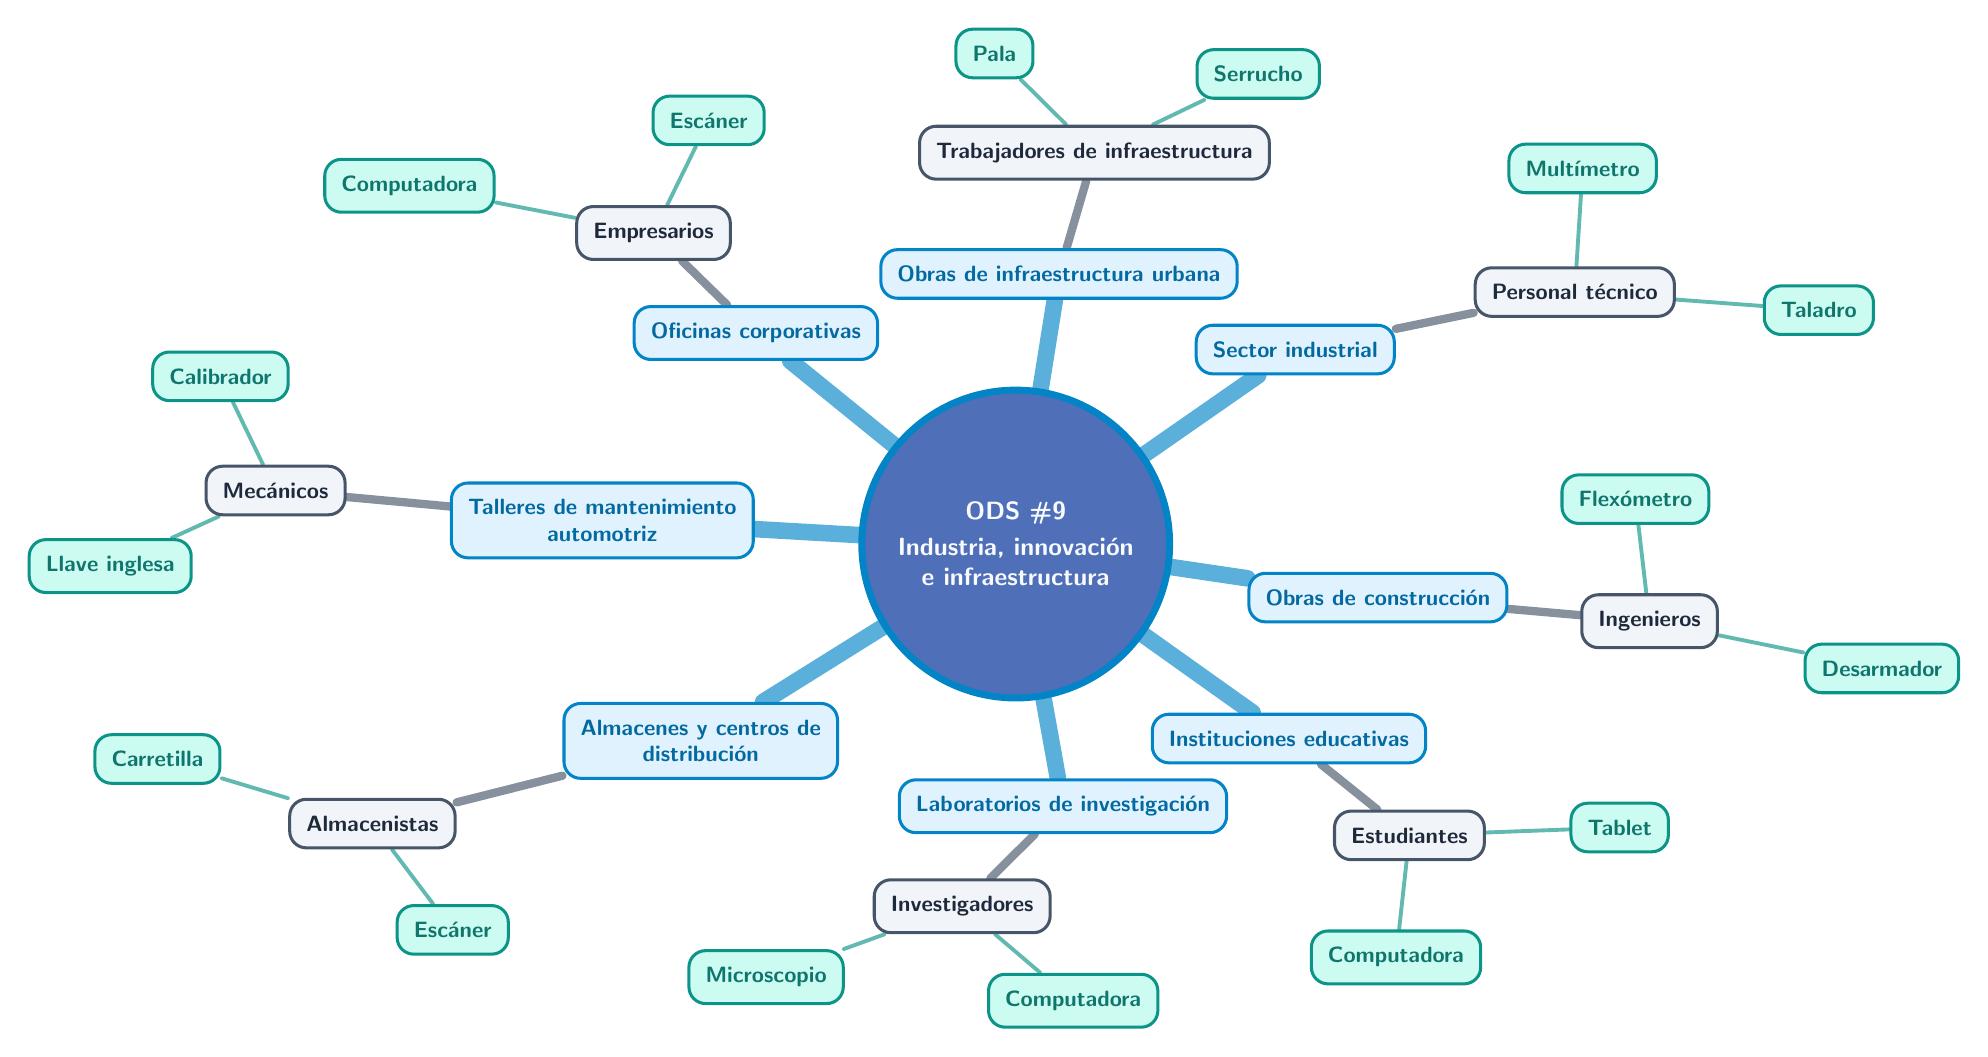
\begin{tikzpicture}[
    root/.style={
      circle,
      fill=lvlRootBg,
      draw=lvlRootBorder,
      line width=2.5pt,
      text=lvlRootText,
      align=center,
      font=\sffamily\bfseries\small,
      inner sep=8pt
    }
  ]

  \node[root] (R) at (0,0) {\textbf{ODS \#9}\\[2pt] Industria, innovación\\e infraestructura};
  \nd{s1}{3.55,2.47}{Sector industrial}{lvlSector}
  \nd{s2}{7.1,3.2}{Personal técnico}{lvlRole}
  \nd{s3}{7.2,4.77}{Multímetro}{lvlTool}
  \nd{s4}{10.2,2.97}{Taladro}{lvlTool}
  \nd{c1}{4.6,-0.68}{Obras de construcción}{lvlSector}
  \nd{c2}{8.05,-0.98}{Ingenieros}{lvlRole}
  \nd{c3}{7.87,0.57}{Flexómetro}{lvlTool}
  \nd{c4}{11,-1.58}{Desarmador}{lvlTool}
  \nd{e1}{3.47,-2.47}{Instituciones educativas}{lvlSector}
  \nd{e2}{5,-3.7}{Estudiantes}{lvlRole}
  \nd{e3}{7.67,-3.6}{Tablet}{lvlTool}
  \nd{e4}{4.83,-5.25}{Computadora}{lvlTool}
  \nd{l1}{0.6,-3.33}{Laboratorios de investigación}{lvlSector}
  \nd{l2}{-0.68,-4.6}{Investigadores}{lvlRole}
  \nd{l3}{-3.17,-5.5}{Microscopio}{lvlTool}
  \nd{l4}{0.73,-5.8}{Computadora}{lvlTool}
  \nd{a1}{-4,-2.5}{Almacenes y centros de\\distribución}{lvlSector}
  \nd{a2}{-8.17,-3.55}{Almacenistas}{lvlRole}
  \nd{a3}{-10.9,-2.73}{Carretilla}{lvlTool}
  \nd{a4}{-7.15,-4.9}{Escáner}{lvlTool}
  \nd{t1}{-5.25,0.3}{Talleres de mantenimiento\\automotriz}{lvlSector}
  \nd{t2}{-9.4,0.68}{Mecánicos}{lvlRole}
  \nd{t3}{-10.1,2.13}{Calibrador}{lvlTool}
  \nd{t4}{-11.5,-0.28}{Llave inglesa}{lvlTool}
  \nd{o1}{-3.3,2.68}{Oficinas corporativas}{lvlSector}
  \nd{o2}{-4.6,3.95}{Empresarios}{lvlRole}
  \nd{o3}{-7.7,4.55}{Computadora}{lvlTool}
  \nd{o4}{-3.9,5.38}{Escáner}{lvlTool}
  \nd{u1}{0.55,3.43}{Obras de infraestructura urbana}{lvlSector}
  \nd{u2}{1.0,4.97}{Trabajadores de infraestructura}{lvlRole}
  \nd{u3}{-0.27,6.23}{Pala}{lvlTool}
  \nd{u4}{3.08,5.97}{Serrucho}{lvlTool}

  \begin{pgfonlayer}{bg}
    \foreach \p in {s,c,e,l,a,t,o,u}{
      \conn{lvlSector}{R}{\p1}{}{6}
      \conn{lvlRole}{\p1}{\p2}{}{3}
      \conn{lvlTool}{\p2}{\p3}{}{1.4}
      \conn{lvlTool}{\p2}{\p4}{}{1.4}
    }
  \end{pgfonlayer}

  \end{tikzpicture}%
  }
  \end{center}
  \caption{Mapa mental de los distintos sectores, roles y herramientas que se verían beneficiados con el proyecto.}
  \label{fig:mapa-mental}
\end{figure}

\begin{multicols*}{2}
Utilizando dicho mapa mental, y haciendo énfasis en la rama del sector industrial. Le daremos forma a nuestro proyecto, el cuál se enfocará en la creación de un sistema de gestión de herramientas compartidas para el sector industrial, con el objetivo de optimizar el uso de recursos y fomentar la colaboración entre empresas y estudiantes. A continuación, se muestra la rama de enfoque del proyecto a partir del mapa mental en la figura \ref{fig:rama-enfoque}.

\vspace{1 em}

\begin{figure}[H]
\begin{center}
\resizebox{\linewidth}{!}{%
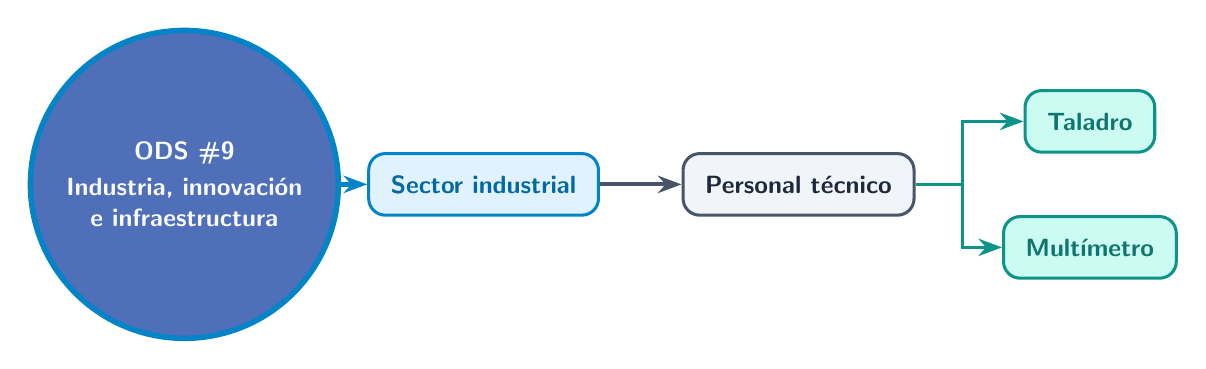
\begin{tikzpicture}[
  font=\sffamily,  
  root/.style={
    circle,
    fill=lvlRootBg,
    draw=lvlRootBorder,
    line width=2pt,
    text=lvlRootText,
    align=center,
    font=\sffamily\bfseries\small,
    inner sep=8pt
  },  
  sector/.style={
    rectangle,
    rounded corners=6pt,
    fill=lvlSectorFill,
    draw=lvlSectorBorder,
    text=lvlSectorText,
    line width=1.1pt,
    align=center,
    font=\sffamily\bfseries\small,
    inner sep=8pt
  },  
  role/.style={
    rectangle,
    rounded corners=6pt,
    fill=lvlRoleFill,
    draw=lvlRoleBorder,
    text=lvlRoleText,
    line width=1.1pt,
    align=center,
    font=\sffamily\bfseries\small,
    inner sep=8pt
  },
  tool/.style={
    rectangle,
    rounded corners=6pt,
    fill=lvlToolFill,
    draw=lvlToolBorder,
    text=lvlToolText,
    line width=1.1pt,
    align=center,
    font=\sffamily\bfseries\small,
    inner sep=8pt
  },  
  arrSector/.style={-{Stealth[length=3mm, width=2.2mm]}, lvlSectorBorder, line width=2pt},
  arrRole/.style={-{Stealth[length=3mm, width=2.2mm]}, lvlRoleBorder, line width=1.5pt},
  arrTool/.style={-{Stealth[length=3mm, width=2.2mm]}, lvlToolBorder, line width=1.2pt}
]

  \node[root] (R) at (0,0) {\textbf{ODS \#9}\\[2pt] Industria, innovación\\e infraestructura};
  \node[sector] (S1) at (3.8,0) {Sector industrial};
  \node[role] (R1) at (7.8,0) {Personal técnico};  
  \node[tool] (T1) at (11.5,0.8) {Taladro};
  \node[tool] (T2) at (11.5,-0.8) {Multímetro};

  \draw[arrSector] (R) -- (S1);
  \draw[arrRole] (S1) -- (R1);
  \draw[arrTool] (R1.east) -- ++(0.6,0) |- (T1);
  \draw[arrTool] (R1.east) -- ++(0.6,0) |- (T2);

\end{tikzpicture}%
}
\caption{Rama de enfoque del proyecto a partir del mapa mental.}
\label{fig:rama-enfoque}
\end{center}
\end{figure}
\vspace{1 em}